\chapter{Standing Wave Pattern}\label{lec:lec5}
In the previous chapter, we introduced the concept of a lossless transmission line (that is a line is lossless if $R=G=0$). We also introduced the concept of a low-loss transmission line which is a more practical transmission line, that is, $R \ll \omega L$, $G \ll \omega C $.

In this chapter, we would study the conditions for treating the transmission line as low-loss at a particular frequency, the variation of voltage and current along a transmission line, the concept of voltage standing wave ratio (VSWR), the condition for full reflection at the load end, the relationship between $R_{\max}$ and VSWR and also the relationship between $R_{\min}$ and VSWR.

\section{Low-loss Transmission Line at a Particular Frequency.}
From our previous chapter, we recall that,
\begin{equation}
\gamma = \frac{1}{2}R\sqrt{\frac{C}{L}} + \frac{G}{2}\sqrt{\frac{L}{C}} +\jmath\omega\sqrt{LC}
\label{eqn:refcoeffient1}
\end{equation}
which states the conditions defined for a low-loss transmission line in terms of the primary constants (R, L, C and G) of the line. To treat a line as a low-loss transmission line, one will have to express these conditions ( $R \ll \omega L$ and $G \ll \omega C$) in terms of the secondary parameters ($\alpha$ and $\beta $) since these parameters are readily available on the data-sheet. If we can establish a relationship between these parameters ($\alpha$ and $\beta $) for the low-loss nature of the line, then we can find out whether a particular line is low-loss at a particular frequency.

Recall that,
\begin{equation}
\gamma = \alpha + \jmath\beta
\label{eqn:refcoeffient2}
\end{equation}
comparing equation~\ref{eqn:refcoeffient1} with equation~\ref{eqn:refcoeffient2}, we have that;
\begin{equation}
\alpha = \frac{1}{2}R\sqrt{\frac{C}{L}} + \frac{1}{2}G\sqrt{\frac{L}{C}}	
\label{eqn:attenconst}
\end{equation}
\begin{align}
\beta = \omega\sqrt{LC}
\end{align}
Since we have expressed equation~\ref{eqn:refcoeffient1} in terms of primary constants, let's find out under what condition the transmission line can be treated as low-loss.

From equation~\ref{eqn:attenconst} we have,
\begin{equation*}
\alpha =\frac{1}{2}R\sqrt{\frac{C}{L}} + \frac{1}{2}G\sqrt{\frac{L}{C}}	
\end{equation*}\\
Multiplying the numerator and denominator of the first term by $\sqrt{\frac{L}{L}}$ and the second term by $\sqrt{\frac{C}{C}}$ , we get;
\begin{equation*}
\alpha = \frac{1}{2} R \sqrt{\frac{C}{L}} \sqrt{\frac{L}{L}} + \frac{1}{2} G \sqrt{\frac{L}{C}} \sqrt{\frac{C}{C}} 
\end{equation*}\\
\begin{equation*}
\alpha =  \frac{1}{2} R \sqrt{\frac{CL}{L^2}} + \frac{1}{2} G \sqrt{\frac{LC}{C^2}}	
\end{equation*}\\
\begin{equation*}
\alpha = \frac{1}{2} \frac{R}{L} \sqrt{LC} + \frac{1}{2} \frac{G}{C} \sqrt{LC}
\end{equation*}\\
Multiplying numerator and denominator by $\omega$\\
\begin{equation*}
\alpha = \frac{1}{2} \frac{R}{\omega L} \omega \sqrt{LC} + \frac{1}{2} \frac{G}{\omega C} \omega \sqrt{LC}
\end{equation*}
\begin{equation*}
\alpha = \frac{1}{2} \omega\sqrt{LC}\left(\frac{R}{\omega L} + \frac{G}{\omega C}\right)
\end{equation*}
But $\beta = \omega \sqrt{LC}$\\
\begin{equation}
\alpha = \beta\frac{1}{2} \left(\frac{R}{\omega L} + \frac{G}{\omega C}\right)
\end{equation}
Recall that for low-loss, $R \ll \omega L$ and $G \ll \omega C$\\
$\frac{R}{\omega L} \ll 1$ and $\frac{G}{\omega C} \ll 1$\\
Therefore,  $\frac{1}{2} (\frac{R}{\omega L} + \frac{G}{\omega C}) \ll 1$\\

$\alpha = \beta \;\; \times$ (something far smaller than 1).\\
Hence, for a low-loss transmission line, $\alpha \ll \beta$ where $\beta = \frac{2 \pi}{\lambda}$.
Considering a wave which travels a distance of one wavelength along the transmission line, its phase change$(\beta)$ becomes $2\pi$ i.e $\beta= 2 \pi$, then the amplitude of the wave varies by:
\begin{equation*}
e^{-\alpha x} = e^{-\alpha \lambda}	
\end{equation*}
Where $\lambda = \frac{2 \pi}{\beta}$
\begin{equation*}
e^{- \alpha x} = e^{-\alpha \frac{2 \pi}{\beta}}
\end{equation*}
Since for a low-loss transmission line $\alpha\ll\beta$, therefore the quantity $e^{-\alpha \frac{2 \pi}{\beta}} \approx 1$.\\\\
Hence, amplitude reduction is very small as the original amplitude is close to the final amplitude. So, a line can be treated as a low-loss transmission line if the change in amplitude over one wavelength is negligibly small. Let our negligibly small be 1 percent change from the original or starting amplitude. Then;\\\\ 
$\frac{\alpha 2 \pi}{\beta} \approx \frac{1}{100}$, $ e^{-0.01} = 0.99005$ of the initial value.\\\\
The wave amplitude only reduces by $1-0.99005=0.00995$ or 1 per cent. That means the wave amplitude only reduces by 1 per cent after a distance of 1 wavelength.\\\\
A line can be treated as a low-loss transmission line if $\alpha \ll \beta$ depending on the given frequency but if the frequency changes such that $\alpha \geq \beta$, the line cannot be treated as a low-loss transmission line.\\

\begin{exmp}
Let's say we have a transmission line with $L = 0.25\mu H/m$, ${C= 100pF/m}$, $G = 0$, what is the resistance of the transmission line so that the line can be treated as a low-loss transmission line given the frequency of operation as $100MHz$ ?\\\\
\textbf{Solution}:\\
$L= 0.25\mu H/m$, $C= 100pF/m$, $G = 0$\\
$\beta = 2\pi \ f {\sqrt{LC}}$
\begin{equation*}
=2 \pi \times 10^8 \sqrt{(0.25 \times 10^{-6}) \times (100 \times 10^{-12})}  = \pi rad/m
\end{equation*}\\
For a low-loss transmission line, taking 1 percent of $\beta$,
$ \alpha= \frac{1}{100} \beta = \frac{\pi}{100}$.\\\\
Also,
\begin{equation*}
\alpha = \beta\frac{1}{2} ( \frac{R}{\omega L} + \frac{G}{\omega C})
\end{equation*}\\
Given that, G=0\\
\begin{equation*}
\alpha = \beta\frac{1}{2} ( \frac{R}{\omega L} )
\end{equation*}\\
Recall that $\beta = \omega\sqrt{LC} $, now we get :
\begin{equation*}
\alpha = \frac{1}{2}\frac{R}{\omega L} \times \omega\sqrt{LC} 
\end{equation*}
\begin{equation*}
\alpha = \frac{1}{2} R \sqrt \frac{LC}{L^{2}} 
\end{equation*}\\
\begin{equation*}
\alpha = \frac{1}{2} R \sqrt \frac{C}{L}
\end{equation*}
\begin{equation*}
\frac{\pi}{100} = \frac{1}{2} R \sqrt{\frac{100 \times 10^{(-12)}}{0.25 \times 10^{(-6)}}}
\end{equation*}
\begin{equation*}
R=\pi\Omega/m.
\end{equation*}\\
If $R \leq \pi\Omega/m$, the line is low-loss at $ f= 100MHz$. If the frequency changes, the line may not satisfy this low-loss condition, hence we have to check again.
\end{exmp}

Therefore, unless you are specifically told that a line is a lossy line, we are at liberty to treat the line as a lossless line since the phase constant as we have seen for lossy and lossless lines are the same. Also, the characteristics impedance of a low-loss line is almost real and the same as the characteristics impedance of a lossless line. So unless we are specifically told the line is lossy, we shall default to treating transmission line problems as lossless and carry out all analysis for a lossless transmission line. Hence for all transmission line problems, we consider it lossless so that, 
\begin{align*}
Z_0 = \sqrt{{\frac{\jmath\omega L}{\jmath\omega C}}} = \sqrt{\frac{L}{C}} = real , \quad \quad \gamma= \jmath\beta = \jmath\omega\sqrt{LC}
\end{align*}

\section{Voltage And Current Variation on Transmission Line}

Revisiting the general voltage and current expression of the transmission line with origin  at the load point, we have:
\begin{equation}
V =  V^+ e^{- \gamma x} + V^- e^{\gamma x}
\label{eqn:genvoltage}
\end{equation}
\begin{equation}
I= \frac{V^+}{Z_o} e^{- \gamma x} - \frac{V^-}{Z_o} e^{\gamma x}
\label{eqn:gencurrent}
\end{equation}
\begin{figure}[h]
\centering
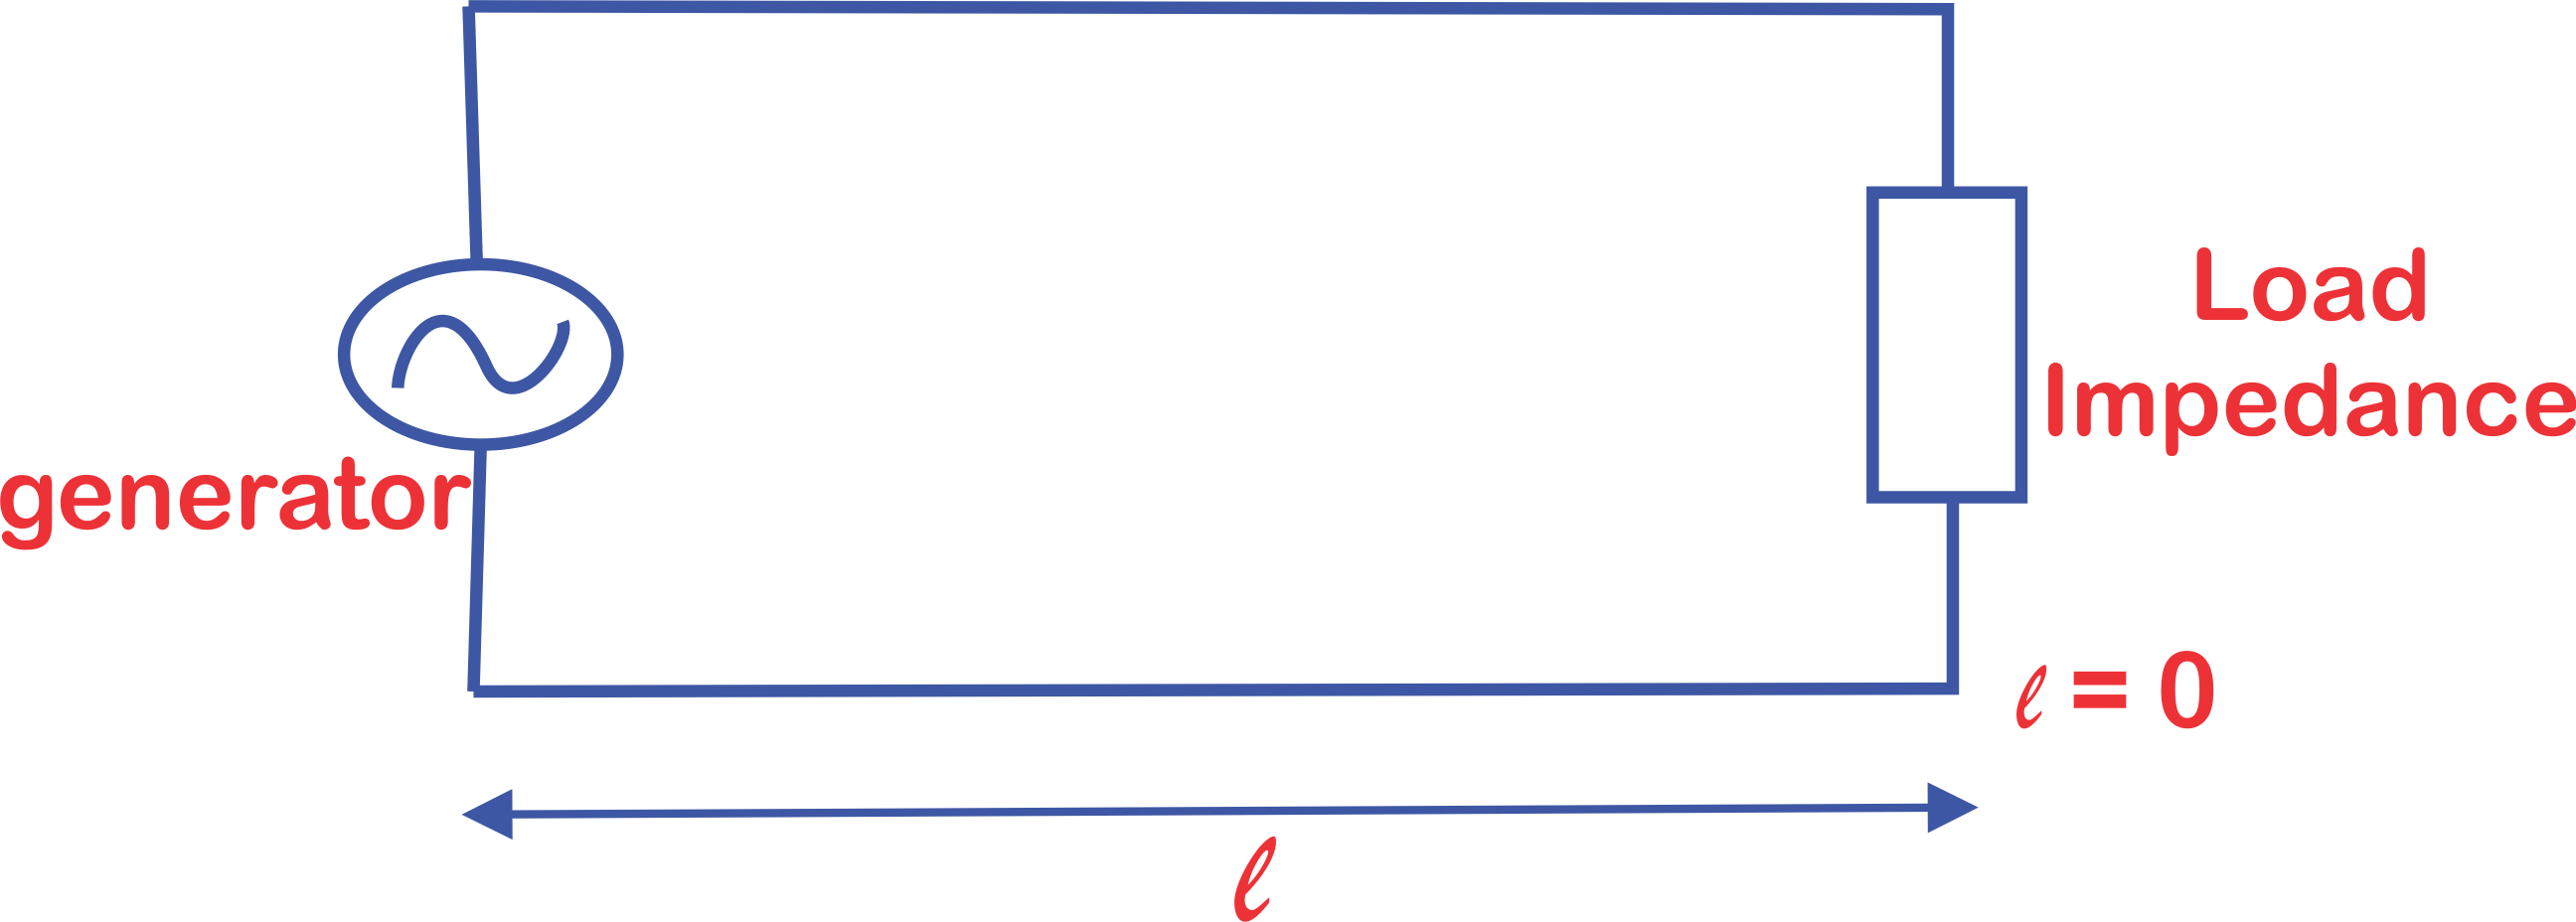
\includegraphics[width=0.9\linewidth]{./graphics/11111111}
\caption{Wave moving towards the Generator}
\label{fig:11111111}
\end{figure}

For a lossless transmission line at any point $l$,\\
substituting $\gamma = \jmath\beta$ and $x=-l$ into equation~\ref{eqn:genvoltage} , we have ;
\begin{equation*}\\
V(l) = V^+ e^{j \beta l} + V^- e^{- j \beta l}
\end{equation*}\\
Divide through by $ V^+ e^{j \beta l}$, we get ;\\
\begin{equation*}
\frac{V(l)}{ V^+ e^{j \beta l}}= (1 +\frac{V^- e^{- j \beta l}}{V^+ e^{j \beta l}})
\end{equation*}\\
\begin{equation*}
V(l) = V^+ e^{j \beta l}(1+ \frac{V^-}{V^+}e^{-j 2 \beta l})
\end{equation*}\\
\begin{equation}
V(l) = V^+ e^{j \beta l}(1 + \Gamma_L e^{-j 2 \beta l})
\label{eqn:voltagefromload}
\end{equation}
where $\Gamma _L = \frac{V^-}{V^+}$. Similarly, substituting $\gamma = j\beta$ and $x = -l$ into equation~\ref{eqn:gencurrent}:
\begin{equation*}
I(l) = \frac{V^+}{Z_o}  e^{\jmath \beta l} - \frac{V^-}{Z_o} e^{-\jmath\beta l}
\end{equation*}
Divide through by $\frac{V^+}{Z_o}  e^{\jmath\beta l}$
\begin{equation*}
\frac{I(l)}{\frac{V^+}{Z_o}  e^{\jmath\beta l}} =( 1- \frac{\frac{V^-}{Z_o} e^{-\jmath\beta l}}{\frac{V^+}{Z_o}  e^{\jmath\beta l}} )
\end{equation*}
\begin{equation*}
\frac{I(l)}{\frac{V^+}{Z_o}  e^{\jmath\beta l}} =( 1-  \frac{V^-}{V^+}e^{-\jmath 2 \beta l})
\end{equation*}
\begin{equation}
I(l) = \frac{V^+}{Z_o}e ^{j \beta l}  \{ 1 - \Gamma_L e^{-j 2 \beta l}\}
\label{eqn:currentfromload}
\end{equation}
where,
\begin{equation*}
\Gamma _L = \frac{V^-}{V^+}
\end{equation*}
$V = f( V^{+}, V^{-})$ and $I = f(I^{+}, I^{-})$ means $V$ and $I$ are a superposition of forward and backward travelling wave, which is then a \textbf{Standing Wave}. 
\begin{equation}
\Gamma_L = |\Gamma_L|e^{j\phi_L}
\label{eqn:refcoefficientfromload}
\end{equation}
where $\phi_L =$ phase of the reflection coefficient at the load end. Then, we can write down the $V(l)$ and $I(l)$ explicitly in terms of the magnitude of the reflection coefficient and the phase.\\
Therefore substituting equation~\ref{eqn:refcoefficientfromload} into equations \ref{eqn:voltagefromload} and \ref{eqn:currentfromload} respectively, we will get ;
\begin{equation*}
V(l) = V^{+}e^{\jmath\beta l}(1 + |\Gamma_L|e^{j\phi_L} . e^{-j 2 \beta l})
\end{equation*}
\begin{equation}
V(l) = V^{+}e^{\jmath\beta l}(1 + |\Gamma_L|  e^{\jmath(\phi_L -2 \beta l)})
\end{equation}
Similarly,
\begin{equation*}
I(l) = \frac{V^+}{Z_o}e ^{j \beta l}( 1 - |\Gamma_L|e^{\jmath\phi_L} . e^{-\jmath 2\beta l})
\end{equation*}
\begin{equation}
I(l) = \frac{V^+}{Z_o}e ^{j \beta l}( 1 -|\Gamma_L|  e^{j(\phi_L -2 \beta l)})
\end{equation}
As we move from load to generator, $l$ increases positively, making $\phi_L -2 \beta l$ more and more negative. In the complex plane, when a phase gets more negative, it means we are moving in a clockwise direction as shown in figure~\ref{fig:473-drawings}.
\begin{figure}[h]
\centering
\includegraphics[width=1\linewidth]{./graphics/"473 drawings"}
\caption{Clockwise and Anticlockwise movement of l}
\label{fig:473-drawings}
\end{figure}

So by moving towards the generator, the phase becomes more and more negative, while the amplitude of $|\Gamma_L|$ remains constant. The total voltage is scaled by the vector sum of the real term (1) and complex term $|\Gamma_L|  e^{j(\phi_L -2 \beta l)}$. Hence, we have a summation of a real vector, whose magnitude is 1, plus a complex term shown below. 
\begin{figure}[h]
\centering
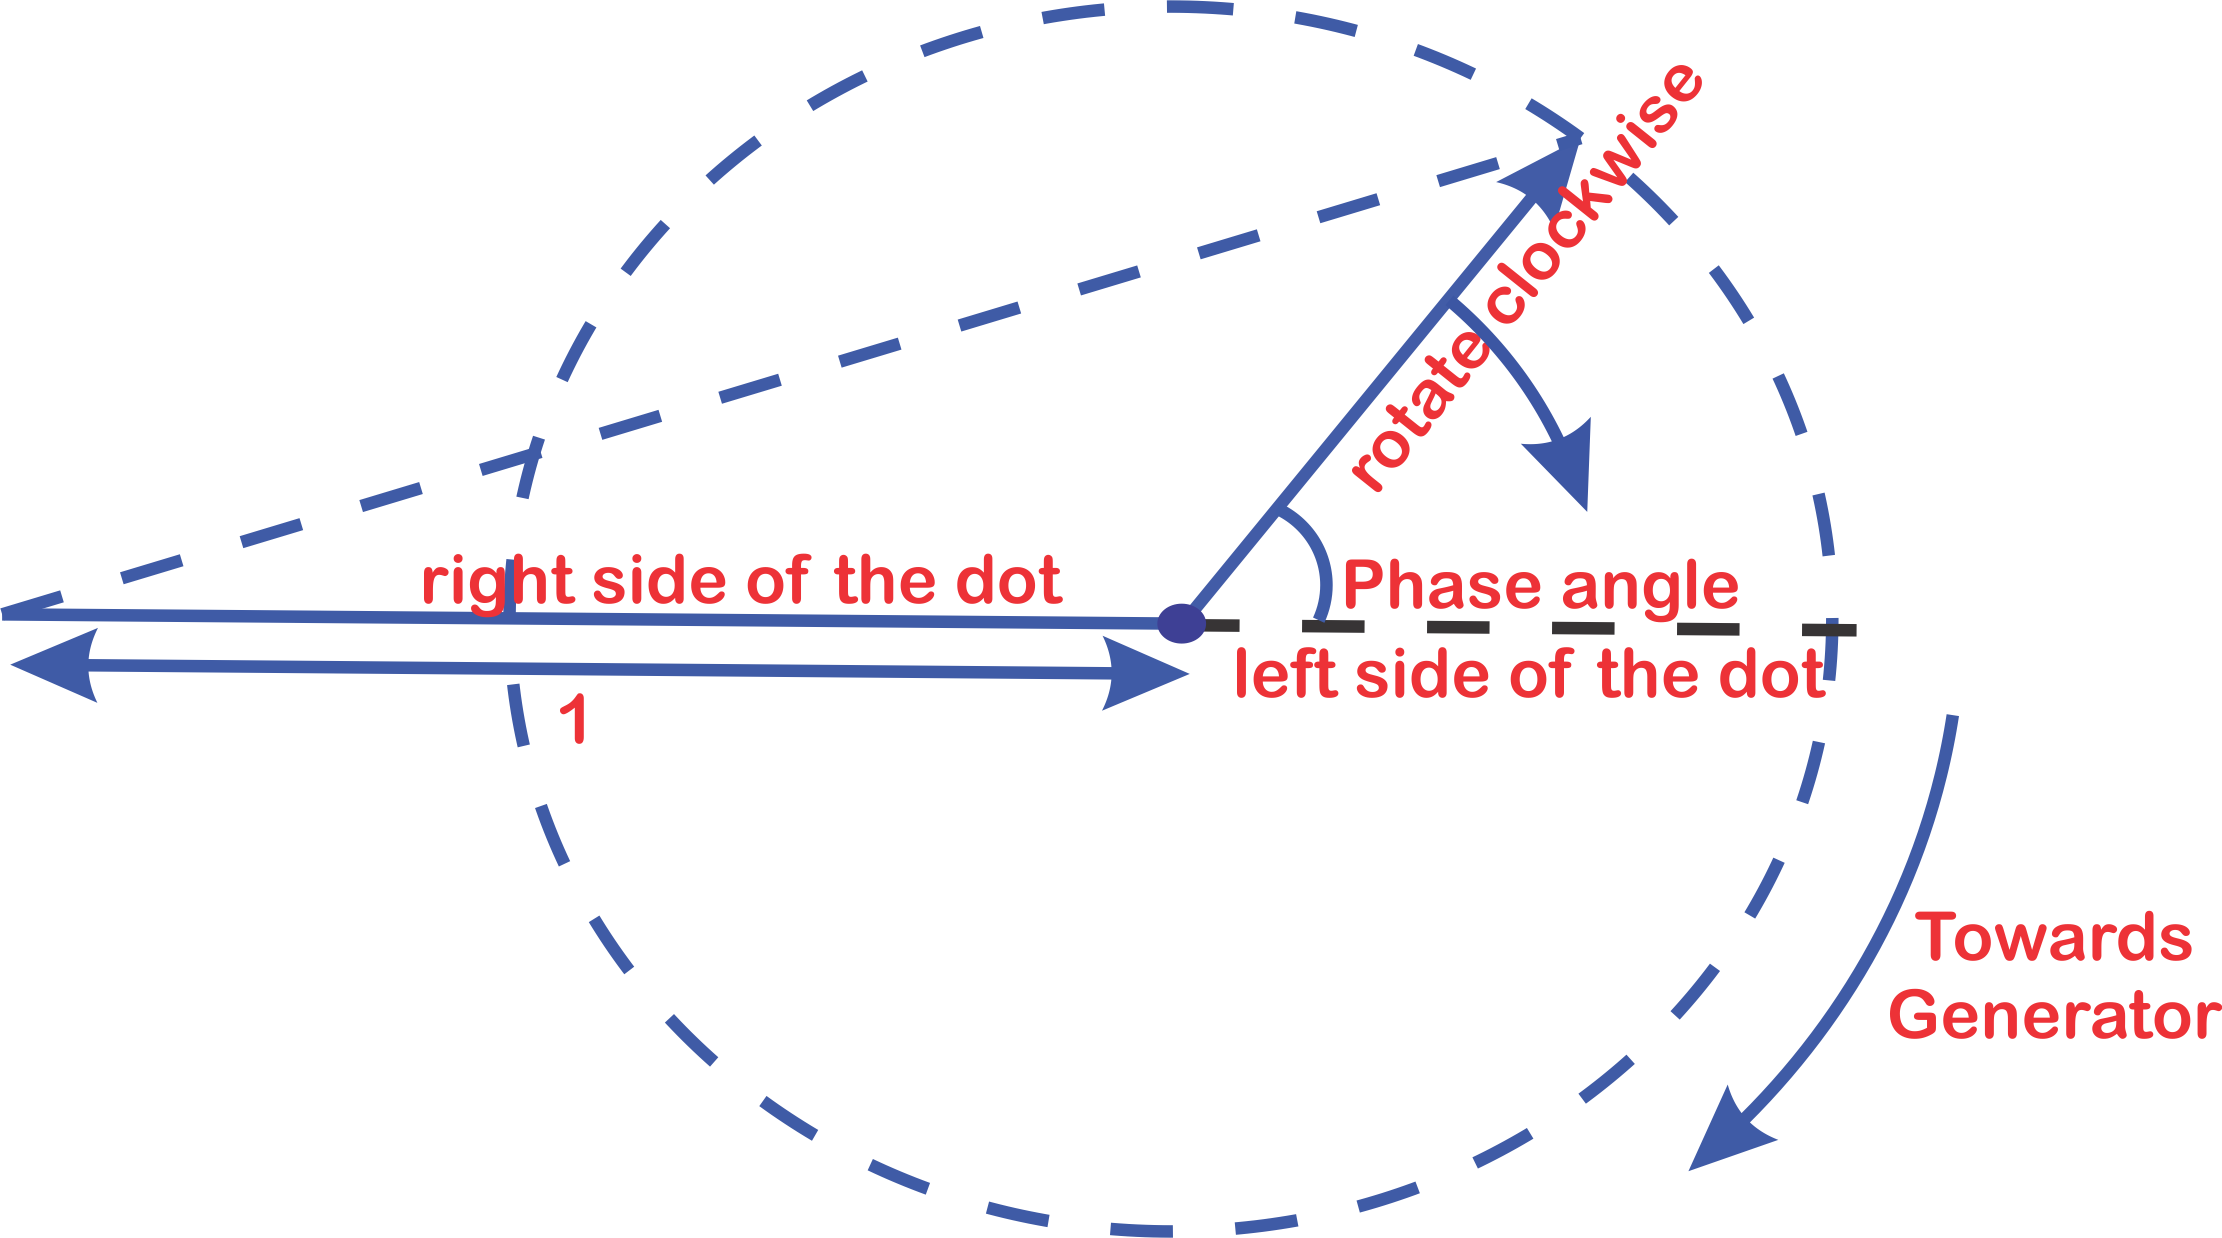
\includegraphics[width=0.8\linewidth]{./graphics/kjhgfdwert}
\caption{Argand Diagram}
\label{fig:kjhgfdwert}
\end{figure}

The magnitude $( 1+|\Gamma_L|  e^{j(\phi_L -2 \beta l)})$ varies as we move along the transmission line.\\
From figure 5.3 \footnote{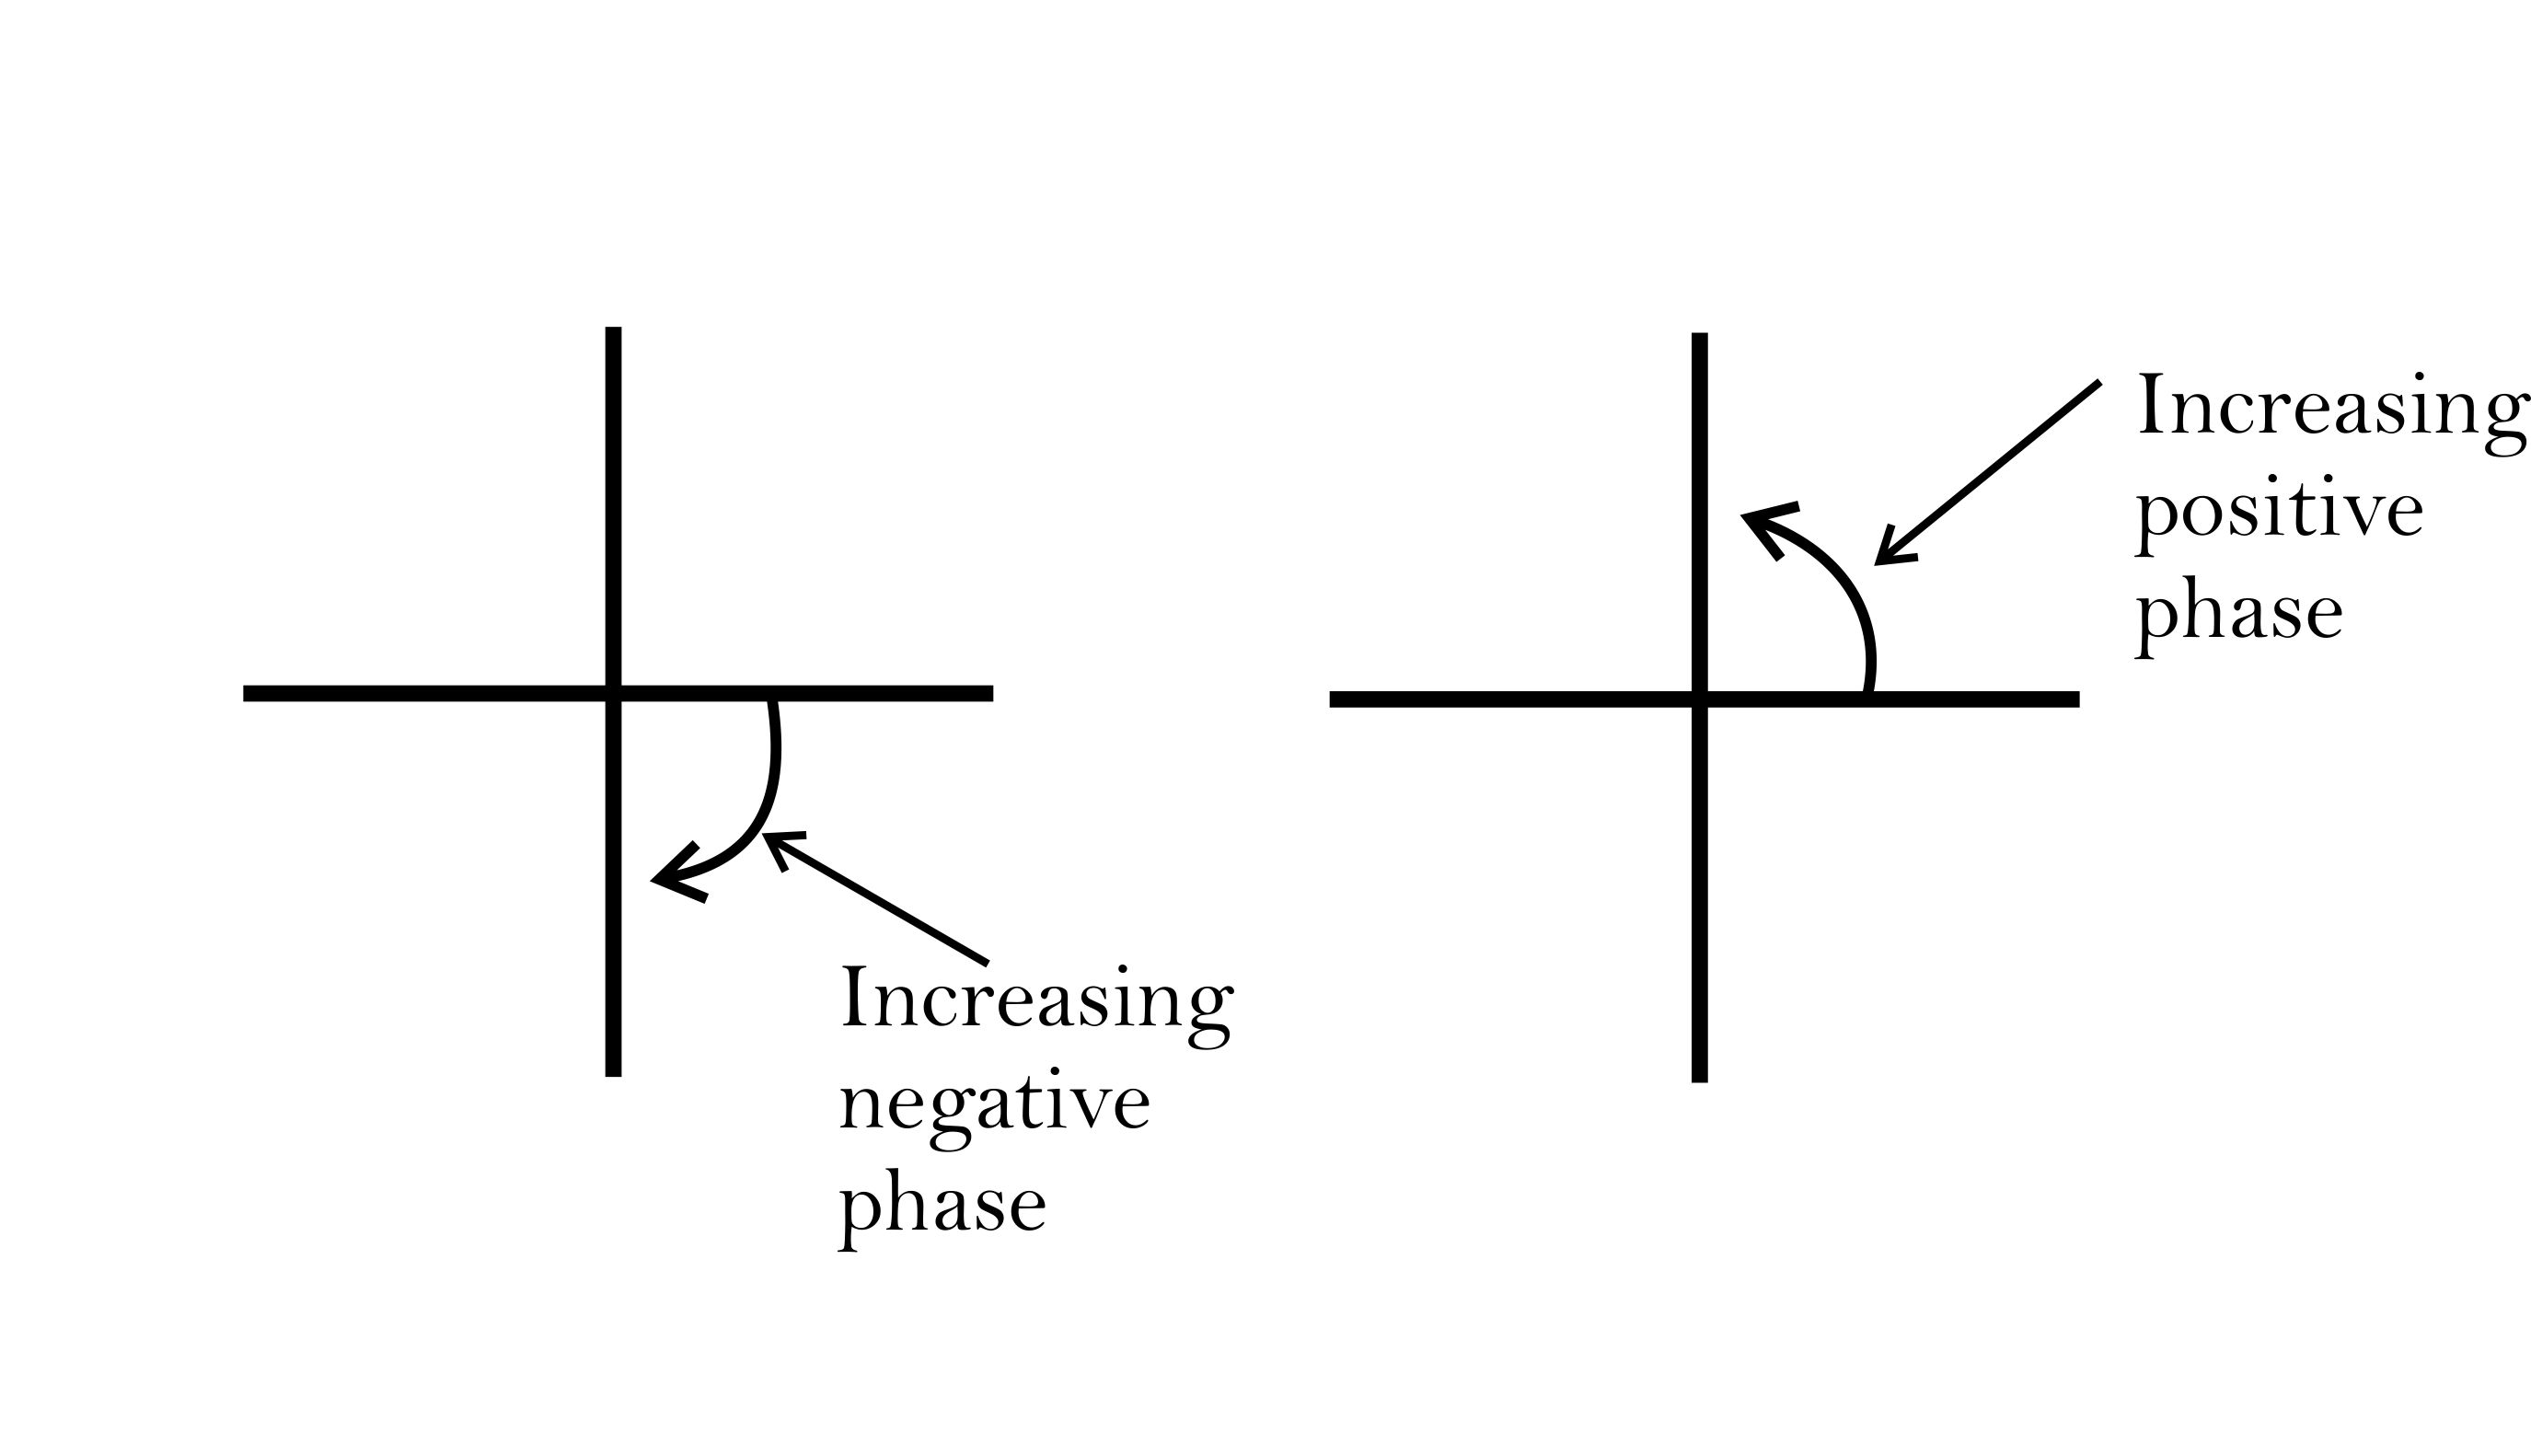
\includegraphics[scale=0.15]{./graphics/picture4} 

Argand Diagram refers to a geometric plot of complex numbers as points z = x+iy using the x-axis as the real axis and the y-axis as the imaginary axis. Such plots are named after Jean-Robert Argand(1768-1822), although they were first described by Norwegian-Danish land surveyor and mathematician Casper Wessel (1745-1818.)}Argand Diagram below, \\
$ A =| 1+| \Gamma_L| e^{j (\phi_L - 2\beta l)}|$ \quad$, B=| \Gamma_L|$\\\\
$Phase\ angle = \phi_L - 2 \beta l$.\\\\
If $ \phi_L - 2 \beta l = 2 \pi n$, where n is an integer, then $ e^{j(\phi_L - 2 \beta l)} = 1$. This is the right side of the dot on the real axis.\\\\ 
Also, if $\phi_L - 2 \beta l=(2 n + 1) \pi$, then $e^{j (\phi_L - 2 \beta l)} = -1$. This is the left side of the dot on the real axis.
\begin{equation*}
V(l) = V^{+}e^{j\beta l}(1 + |\Gamma_L|  e^{j(\phi_L -2\beta l)})
\end{equation*}
$(1 + |\Gamma_L|  e^{j(\phi_L -2\beta l)})$ add when they are in phase to give maximum V i.e at $(\phi_L -2\beta l) = 0, 2\pi, 4\pi ...$, and subtract to give minimum V i.e at  $(\phi_L -2\beta l) = \pi, 3\pi, 5\pi ...$ \\
This is opposite to the behaviour of the current relationship, when 1 and  $-|\Gamma_L|  e^{j(\phi_L -2\beta l)}$ in $1-|\Gamma_L|  e^{j(\phi_L -2\beta l)}$ are out of phase, they add at $\pi, 3\pi, 5\pi...$ to give maximum current and they cancel when in phase at $0, 2\pi, 4\pi...$, to give minimum current.\\
As stated earlier, when $ e^{j(\phi_L - 2 \beta l)} = 1$, the voltage is maximum and the current is minimum. When $ e^{\jmath(\phi_L - 2 \beta l)} = -1$, the voltage is minimum and the current is maximum. So at the same location along the transmission line, maximum voltage corresponds to minimum current, and minimum voltage corresponds to maximum current. This is opposite to what we observed in a lumped circuit, where the maximum voltage point corresponds to maximum current and minimum voltage corresponds to minimum current.\\
The maximum voltage and current does not occur at the same point on the transmission line, they are staggered in space. Whenever there is a maximum voltage, there is a minimum current and vice versa. So the standing wave of voltage and current are shifted with respect to each other in space on the transmission line. 
\begin{figure}[h]
\centering
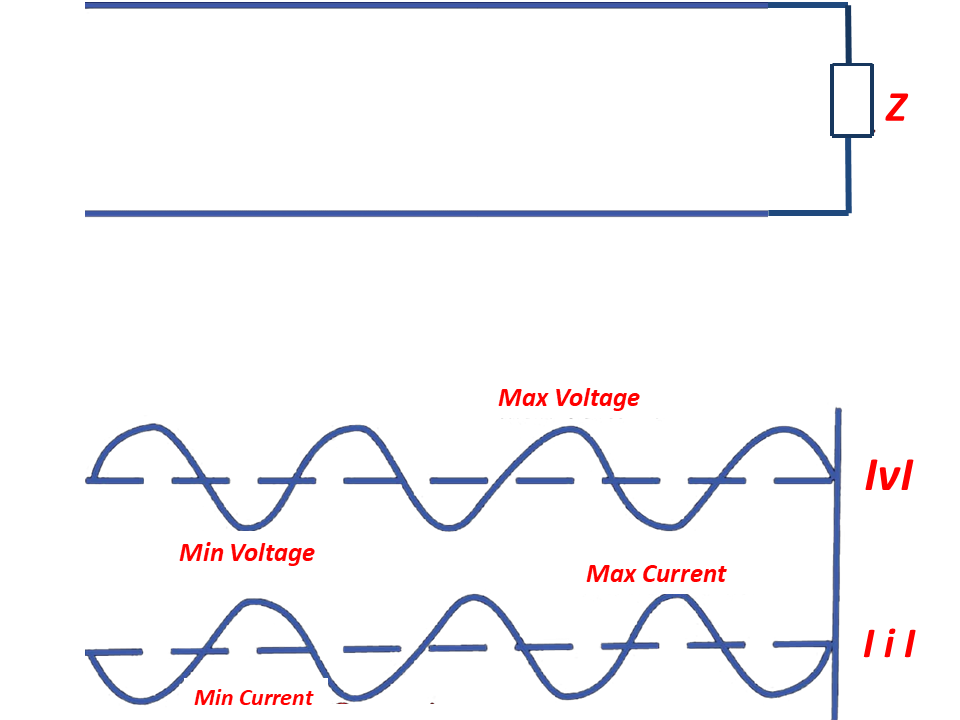
\includegraphics[width=0.7\linewidth]{./graphics/fig5.4modified}
\caption{Voltage and Current Plot, with Increasing l to the left}
\label{fig:asdfghjhgfdsa}
\end{figure}
From figure 5.4, we observe that maximum voltage corresponds to minimum current and minimum voltage corresponds to maximum current.

\section{Concept of Voltage Standing Wave Ratio (VSWR)}
Recall that;
\begin{align*}
\frac{V(l)}{I(l)} = \frac{V^{+}e^{j\beta l}(1+ |\Gamma_L|e^{j(\phi_L- 2 \beta l)})}{\frac{V^{+}}{Z_o}(1- |\Gamma_L|e^{j(\phi_L- 2\beta l)})}
\end{align*}
Therefore,
\begin{equation*}
\frac{V(l)}{I(l)} = Z_o \frac{1+ |\Gamma_L|e^{j(\phi_L- 2 \beta l)}}{1- |\Gamma_L|e^{j(\phi_L- 2\beta l)}}
\end{equation*}
For maximum voltage, $\phi_L-2\beta l = \textnormal{Even multiples of }\pi$ that is $0, 2\pi, 4\pi,  6\pi,\ldots$. For minimum voltage,  $\phi_L-2\beta l=\textnormal{Odd multiples of } \pi$ that is $\pi, 3\pi,\ 5\pi,\ \ldots$. Thus the euler formular 
\[e^{j(\phi_L - 2 \beta l)} = \cos(\phi_L - 2 \beta l) + jsin(\phi_L - 2 \beta l)\]
Since $\sin(\phi_L - 2 \beta l) = 0$ for all multiples of $\pi$ or $n\pi$, where n is an integer becomes real. So when a voltage is maximum or minimum, $\frac{V(l)}{I(l)} = Z_o \times$ (real quantity).

So irrespective of what the line is terminated in at maximum voltage, the impedance at that point is always real. Even if the line is terminated in a complex impedance, the maximum voltage is always real. If we move to the point of maximum voltage, the impedance that will be measured at that point will always be real. Similarly, at the location where the voltage is minimum, the impedance will again be real.

In conclusion, on a transmission line, wherever there is a maximum voltage the impedance measured at that point will be real, same for the point of minimum voltage.

Mathematically, the maximum impedance is expressed as
\begin{equation}
Z_{\max} = \frac{|V_{\max}|}{|I_{\min}|} = R_{\max}
\label{eqn:maximp}
\end{equation}
\begin{equation}
R_{\max}= Z_o\left\{\frac{1+|\Gamma_L|}{1-|\Gamma_L|}\right\}
\end{equation}
At the location of minimum voltage, the minimum impedance is expressed as
\begin{equation}
Z_{\min}=\frac{|V_{\min}|}{|I_{\max}|} = R_{\min}
\label{eqn:minimp}
\end{equation}
\begin{equation}
R_{\min} =Z_o\left\{\frac{1-|\Gamma_L|}{1+|\Gamma_L|}\right\}
\end{equation}
Once load impedance, characteristic impedance $Z_o$ as well as the reflection coefficient $\Gamma_L$ are known, then we can calculate the maximum and minimum value of impedance that we see on the transmission line. As we move along the transmission line, the impedance will vary. However, there is a bound on the upper and lower value of this impedance; the lowest according to Equation~\ref{eqn:maximp} and the lowest according to Equation~\ref{eqn:minimp}.

Once we have the voltage standing wave on the transmission line, at high frequencies the measurement of phase is very difficult and complicated. One can measure the amplitude of a signal reliably but the measurement of phase is rather uncertain. So at high frequencies, we estimate the phase but in a not direct manner rather indirect by measuring only the magnitude quantities. As we have seen the phase of the signal in time gets translated into the space phase because the total phase we see on a wave is a combination of space and time relationship between the two waves, the forward and backward wave. 

These waves are related to the time phase and the space phase ($\omega t + \beta x$) where $\omega t$ is the time phase and $\beta x$ is the space phase. Since the total phase governs the location of maximum and minimum on the standing wave, noting the location of maximum and minimum on the transmission line, one can estimate the phase of the signal. Now we define a parameter for the standing wave which is a parameter of only amplitude variation of the transmission line. This quantity is called the \textbf{Voltage Standing Wave Ratio (VSWR)}\index{voltage standing wave ratio} \emph{which is the measure of the relative contribution of the reflected wave with respect to the incident wave}. If the reflected wave is zero, there is no standing wave but only a travelling wave and if the reflected wave is the same as the transmitted wave, then we have a completely developed standing wave. So the interference of the two waves, the forward and backward wave is going to give the variation of $R_{\max}$ to $R_{\min}$ and $R_{\min}$ to $R_{\max}$. So we define a quantity relating $V_{\max}$ and $V_{\min}$, then $\dfrac{V_{\max}}{V_{\min}}= VSWR$. It is a very important quantity because without carrying out phase measurements, we can measure this quantity on a transmission line. Recall that the reflection coefficient is a complex quantity, so a complete knowledge of the reflection coefficient is achieved when both its amplitude and phase are known. However, the quantity which we are defining is known as VSWR or \(\rho\) which is measured only by amplitude.

Therefore, by measuring the maximum and minimum values of the standing wave, we get;
\begin{dmath*}
VSWR = \rho =\frac{|V|_{\max}}{|V|_{\min}} = \frac{|V^+|\{1+|\Gamma_L|\}}{|V^+|\{1-|\Gamma_L|\}}
\end{dmath*}
\begin{equation}
VSWR  = \frac{1+|\Gamma_L|}{1-|\Gamma_L|}	
\end{equation}

\section{Condition for Full Reflection at Load End}
Since the transmission line is lossless, the reflection coefficient at the load is;
\begin{equation*}
|\Gamma_L| = \frac{Z_L-Z_o}{Z_L+Z_o}
\end{equation*}
$Z_o$ is real for a lossless transmission line, $Z_L$ can have any complex impedance as load but $Z_o$ is real.

So, $	|\Gamma_L| = \frac{Z_L-Z_o}{Z_L+Z_o}$ is always less than 1 that is:
\begin{equation*}
|\Gamma_L|\leq 1\quad  (\textnormal{for  a  passive load})
\end{equation*}
What this means is that $|\Gamma_L|$ is the relative amplitude of the reflected wave with respect to the incident wave and its value no more than 1 implies that we do not have any energy source at the load point so the transmitted energy  can only be reflected. Therefore, the amplitude of the reflected wave has to always be less than or equal to the amplitude of the incident wave.

\subsection{Conditions for which $|\Gamma_L|=1$}
\textbf{Case 1}: $Z_L=0$ (the line is short-circuited at the load end)
\begin{equation*}	
\Gamma_L= \frac{Z_L -Z_o}{Z_L + Z_o} =  \frac{0 -Z_0}{0 + Z_0} = -1	
\end{equation*}
\begin{equation*}
|\Gamma_L|=1
\end{equation*}	
\textbf{Case 2}: $Z_L=\infty$ (Open circuit line)
\begin{equation*}
\Gamma_L= \frac{Z_L -Z_o}{Z_L + Z_o}
\end{equation*}
\begin{equation*}
\Gamma_L = \frac{1 -\frac{Z_o}{Z_L}}{1 + \frac{Z_0}{Z_L}} = \frac{1 - 0}{1 + 0} = 1
\end{equation*}
\begin{equation*}
|\Gamma_L| = 1
\end{equation*}
\textbf{Case 3}: $Z_L = \jmath X$ (Pure reactance)
\begin{equation*}
\Gamma_L= \frac{Z_L -Z_o}{Z_L + Z_o}
\end{equation*}
\begin{equation*}
\Gamma_L = \frac{\jmath X - Z_o}{\jmath X + Z_o} = \textnormal{complex}
\end{equation*}
\begin{equation*}
|\Gamma_L| = 1
\end{equation*}
So the three cases under which $|\Gamma_L|=1$ are
\begin{enumerate}[(i)]
\item When the line is short-circuited.
\item When the line is open-circuited.
\item When the line is terminated in a pure reactance
\end{enumerate}
Since there is no energy-absorbing circuit at the load end of the line, short circuits, open circuits and ideal reactance cannot absorb power. So, whatever power the generator takes to the load end, it has no option but to return all the power in the reflected waveform.
\begin{align*}
VSWR  = \frac{1+|\Gamma_L|}{1-|\Gamma_L|}
\end{align*}
The $VSWR$ will always be greater than 1, the best case is $|\Gamma_L|=0$ (zero reflection) which gives $VSWR=1$ whereas at $|\Gamma_L|=1$ (full reflection), $\rho= \infty$.

So $1\leq\rho\leq\infty$, where $\rho=0$ represents no reflected wave on the transmission line i.e full power is transferred to the load and $\rho = \infty$ means so much reflection on the transmission line or less efficiency of power transfer to the load. So, every circuit design tries to make \(VSWR\) as close to 1 as possible. A higher value of \(VSWR\) indicates more mismatch on the transmission line or a higher value of the reflected wave on the transmission line.

So \(VSWR\) is one of the most important quantities at high frequency. When designing a circuit, we try to make sure the \(VSWR\) on the transmission line is close to one as possible, making sure the circuit is efficiently transferring power to the load end of the line. Once $\rho$ or VSWR is defined, we can relate it to the maximum and minimum impedance that can be seen on the transmission line.

\subsection{Relating $\rho$ to $R_{\max}$ and  $R_{\min}$}
Recall that $\rho =  \left(\frac{1 + |\Gamma_L|}{1 - |\Gamma_L|}\right)$
\begin{equation*}
R_{\max}  = Z_o  \left(\frac{1 + |\Gamma_L|}{1 - |\Gamma_L|}\right) = Z_o    \  \rho
\end{equation*}
\begin{equation*}
R_{\min}  = Z_o  \left(\frac{1 - |\Gamma_L|}{1 + |\Gamma_L|}\right) =\frac{Z_o}{\rho}
\end{equation*}
Therefore
\begin{align}
R_{\max} &= Z_o \rho\label{eqn:maximprho}\\
R_{\min} &= \frac{Z_o}{\rho}\label{eqn:minimpeho}
\end{align}
This implies that for any line terminated with an arbitrary impedance, if we move to a point where the voltage is maximum or minimum, then we know the value of the impedance at that location. Because measuring $V_{\max}$ and $V_{\min}$ gives us $\rho$. $Z_o$ is known beforehand, hence $R_{\max}$ = $Z_o \rho$ and $R_{\min} = \frac{Z_o}{\rho}$.

We know that the impedance known at any point in a transmission line can always be transformed to any other point using the impedance transformation relation. Hence knowing the location at voltage maximum or minimum, since the impedance value is known there, then we can transform the impedance value towards the load to get the load impedance. This essentially opens up a measurement technique for unknown impedance.

At high frequencies, if we have a complex impedance, its measurement is quite tedious because we cannot measure phase accurately. Now we have a mechanism for measuring the phase indirectly. As we have mentioned, the phase gets reflected into the standing wave pattern on the location of voltage maximum and minimum. So if we measure VSWR and the location of $V_{\max}$ and $V_{\min}$ we can always transform $R_{\max}$ or $R_{\min}$ to the location of the load which is nothing but the load impedance. So if we transform from the load impedance to the voltage maximum or minimum we would get $R_{\max}$ and $R_{\min}$. In summary, ig the location of $V_{\max}$ from the load is known and the value of impedance at that location, and the distance of the load from that point are also known, then the transformation of $R_{\max}$ or $R_{\min}$ to load end should give load impedance.

When we go to the application of transmission line we will see that the technique is used for measuring complex impedances. Then we will explicitly derive the expression for the unknown impedance which is terminated to a transmission line. 